\documentclass[11pt,a4paper]{article}
\usepackage{float}
\usepackage{verbatim}
\usepackage{subfig}
\usepackage[T1]{fontenc}
\usepackage[utf8]{inputenc}
\usepackage{geometry}
\usepackage{enumitem}
%\geometry{verbose,lmargin=2cm,rmargin=2cm, bmargin=2cm, tmargin=2cm}
\usepackage{wrapfig}
\usepackage{tikz}
\usetikzlibrary{decorations.markings}
\usepackage{calc}
\usepackage{wrapfig}
\usepackage{graphicx}
\usepackage{amssymb}
\usepackage{amsmath}
\usepackage{esint}
\usepackage{hyperref}
\usepackage{listings}
\lstset{ %
  basicstyle=\footnotesize,        % the size of the fonts that are used for the code
  breakatwhitespace=false,         % sets if automatic breaks should only happen at whitespace
  breaklines=true,                 % sets automatic line breaking
  captionpos=t,                    % sets the caption-position to bottom
  deletekeywords={...},            % if you want to delete keywords from the given language
  escapeinside={\%*}{*)},          % if you want to add LaTeX within your code
  extendedchars=true,              % lets you use non-ASCII characters; for 8-bits encodings only, does not work with UTF-8
  frame=single,                    % adds a frame around the code
  keepspaces=true,                 % keeps spaces in text, useful for keeping indentation of code (possibly needs columns=flexible)
 % language=Python,                 % the language of the code
  morekeywords={*,...},           % if you want to add more keywords to the set
  numbers=left,                    % where to put the line-numbers; possible values are (none, left, right)
  numbersep=5pt,                   % how far the line-numbers are from the code
  showspaces=false,                % show spaces everywhere adding particular underscores; it overrides 'showstringspaces'
  showstringspaces=false,          % underline spaces within strings only
  showtabs=false,                  % show tabs within strings adding particular underscores
  stepnumber=1,                    % the step between two line-numbers. If it's 1, each line will be numbered
  tabsize=2,                       % sets default tabsize to 2 spaces
  title=\lstname                   % show the filename of files included with \lstinputlisting; also try caption instead of title
}
\begin{document}



%\preprint{APS/123-QED}

\title{FYS2150 \\ Lab Report: Elasticity}% Force line breaks with \\

\author{Nicholas Karlsen}
% \email{nichoka@student.matnat.uio.no}

\date{\today}% It is always \today, today,
             %  but any date may be explicitly specified

\maketitle

\begin{abstract}
    A study on two different methods to determine the Young's modulus of a brass rod.
\end{abstract}

%\tableofcontents

\section{\label{sect:intro}Introduction}
    
\section{\label{sect:theory}Theory}
  \subsection{Euler-Bernoulli beam theory}
  \begin{equation}
    h(m) = \frac{mgl^3}{48EI}
  \end{equation}
  \begin{equation}
    E = \frac{4l^3g}{3\pi |A|d^4}
  \end{equation}
  \subsection{Errors}
    When performing arithmetic operations on recorded data, the uncertainty in the data must also carry over to the derived results. How these uncertainties carry over in different operations can be found in Practical Physics \cite{squires}.

\section{\label{section:experimental}Experimental Procedure}
  \subsection{Three-point flexural test}

    \begin{figure}[H]
      \centering
      \subfloat[][]{
        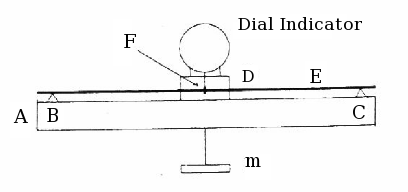
\includegraphics[width=9cm]{scripts/figs/aparatus1.png}
          \label{fig:aparatus1}}
      \subfloat[][]{
        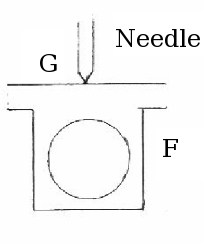
\includegraphics[width=4cm]{scripts/figs/aparatus1cs.png}
          \label{fig:aparatus1cs}}
      \center
      \caption{(a) shows the apparatus used for measuring the deflection of a rod and (b) a cross section of the  aparatus at point F.}
      \label{fig:exp_1}
    \end{figure}

    Using \ref{fig:aparatus1} as a reference; The brass rod, A, was laid on the "knives" B and C. In the middle of the rod, there was a ring as shown in Fig. \ref{fig:aparatus1cs}. The flat surface of the ring was in contact with the needle of the dial indicator at G. In order to ensure that the flat surface of the ring was at right angle with the needle, we turned the rod such that the reading of the dial indicator would be at a minimum, as the skewer the surface, the greater the reading. This process was repeated at the start of every attempt of the experiment.
    
  \subsection{Measuring the speed of sound in the rod}
      The brass rod, with a ring attached to it (same as before), was laid to rest on the flat side of the ring on a solid surface such that the rod is held up by the ring. We also made sure that the rod was not to be disturbed in any way while it was vibrating. When hit with a hammer, it will emit a sound consisting of different frequencies. Following are the two different methods we used for determining the root frequency of the rod.
      During both experiments, we ensured there were no significant noise pollution during our recording (By which i mean people performing the same experiment as us).
      \subsubsection{By hearing for beats}
        A speaker was connected to a signal generator. We started the signal generator at 1200Hz and hit the brass rod with a plastic hammer on the the flat surface on one end of the rod. By ear, there was an audible beat due to the superposition of the two signals. We adjusted the signal generator such that the the frequency of the beat was minimized, and there was essentially no audible difference between the two signals. We did this by trying above and below where we thought the root frequency was, eventually zeroing in on a value.

      \subsubsection{By Fourier transform}
        A USB microphone was placed close to the rod, and faced towards it. The microphone was connected to a computer running matlab, with a script that collects audio data from it and Fourier transforms it using FFT. The recordings made were made with a sampling frequency of $8\times1024$ Hz and varying durations. As before, we hit the rod using a plastic hammer and recorded the data.


\section{\label{sect:results}Results}
  \subsection{Results from Three-point flexural test}


    \begin{table}[H]
      % Measured flex
      \caption{Flex of beam, h(m), with rough m.}
      \center
      \begin{tabular}{ | p{1.2cm} | p{1.4cm} | p{1.4cm} | p{1.4cm} | p{1.4cm} | p{1.4cm} | p{1.4cm} | p{1.4cm} | p{1.4cm} |}
          \hline
          Attempt no. & h(0kg) [mm] & h(0.5kg) [mm] & h(1kg) [mm] & h(1.5kg) [mm] & h(2.0kg) [mm] & h(2.5kg) [mm] & h(3.0kg) [mm] & h(3.5kg) [mm] \\ 
          \hline
          1 & 9.44 & 8.72 & 8.00 & 7.28 & 6.58 & 5.84 & 5.15 & 4.43\\ \hline
          2 & 9.42 & 8.70 & 7.98 & 7.26 & 6.53 & 5.80 & 5.09 & 4.39\\ \hline
          3 & 9.42 & 8.71 & 7.98 & 7.26 & 6.53 & 5.80 & 5.09 & 4.37\\ \hline
          4 & 9.41 & 8.69 & 7.97 & 7.25 & 6.52 & 5.79 & 5.08 & 4.36\\ \hline
          5 & 9.42 & 8.70 & 7.98 & 7.26 & 6.70 & 5.87 & 5.19 & 4.51\\ \hline
      \end{tabular}
      \label{tab:flex}
    \end{table}

   
    \begin{figure}[H]
      \centering
      \subfloat[][Flex of rod]{
        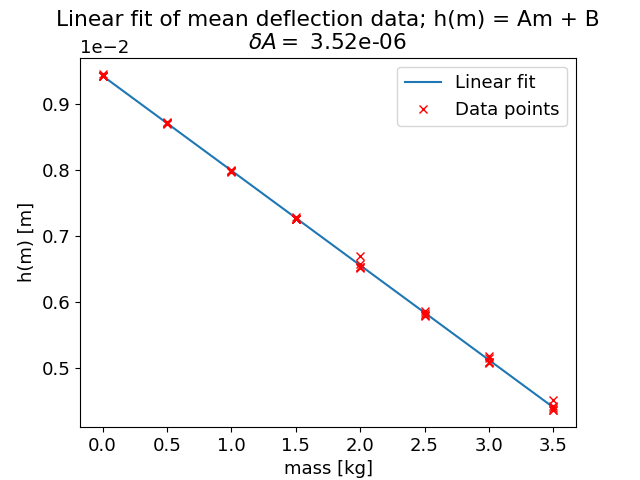
\includegraphics[width=8cm]{scripts/figs/h_m_fig.png}
          \label{fig:h(m)}} 
      \subfloat[][Standard deviation of data]{
        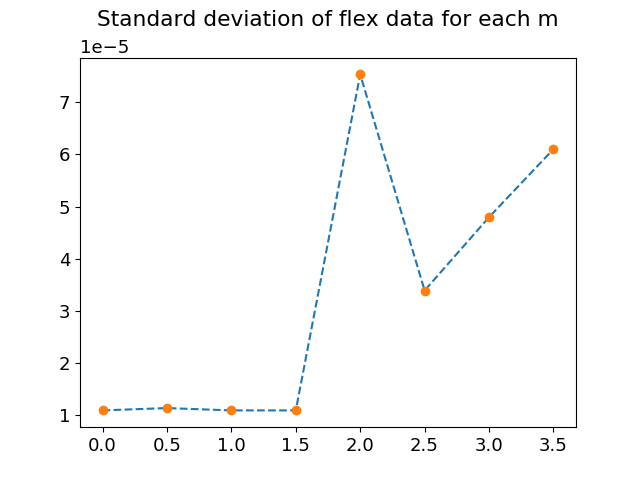
\includegraphics[width=8cm]{scripts/figs/h_m_deviation.png}
          \label{fig:deviation_h_m}}
      \center
      \caption{(a) Shows the flex of the brass beam measured by the dial indicatior. (b) Shows the standard deviation of the data points in (a) at their respective masses}
      \label{fig:exp_1}
    \end{figure}

  Table \ref{tab:flex} contains the data recorded with the dial indicator
  \newline
  \newline
  Fig. \ref{fig:h(m)} contains all the recorded data, as well as a linear fit on the mean of h(m) for each m. The error of the linear fit, $h(m) = Am + B$, $dA = 3.52e-06$.

  \subsection{Results from measuring the speed of sound in the rod}

    When hearing for beats, me and my labpartner decided that the root frequency was $\approx 1240\enspace\textup{Hz}$.
    \newline
    \begin{figure}[H]
      \centering
      \subfloat[][Time domain]{
        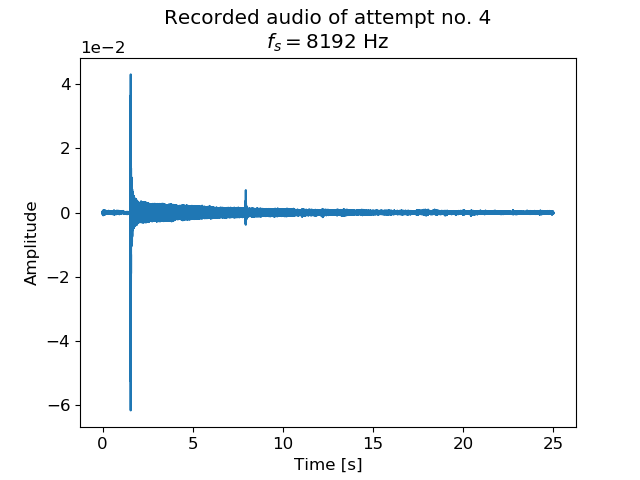
\includegraphics[width=8cm]{scripts/raw_exp2_4.png}
          \label{ }} \\
      \subfloat[][Frequency domain]{
        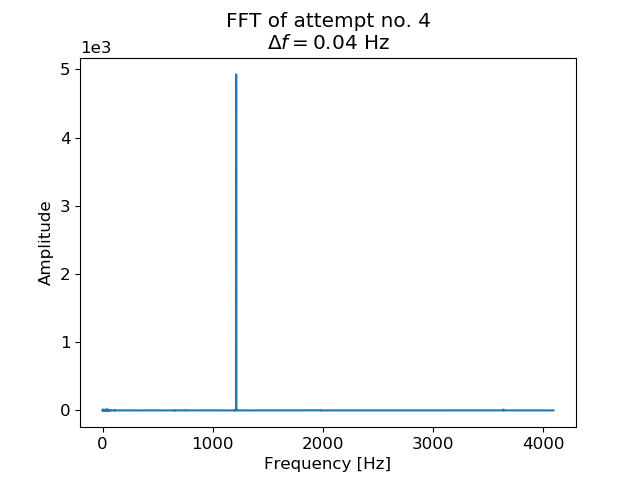
\includegraphics[width=8cm]{scripts/energy_exp2_4.png}
          \label{ }} \\
      \subfloat[][Zoomed frequency domain]{
        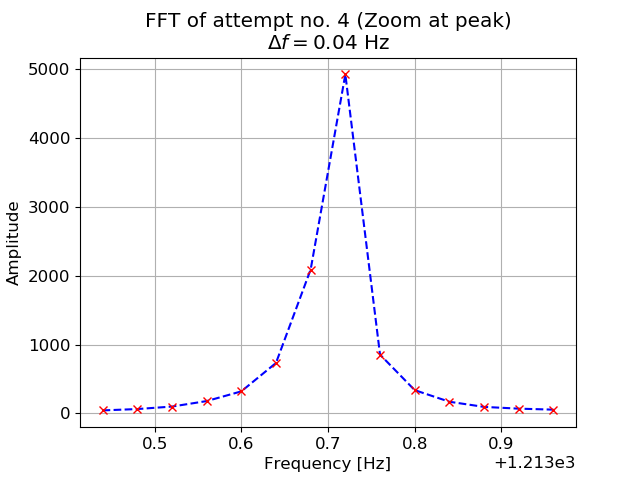
\includegraphics[width=8cm]{scripts/freq_exp2_4.png}
          \label{ }}
      \caption{All of the plots generated for attempt no. 4}
      \label{fig:sound_exp1}
    \end{figure}

    \begin{figure}[H]
      \centering 
      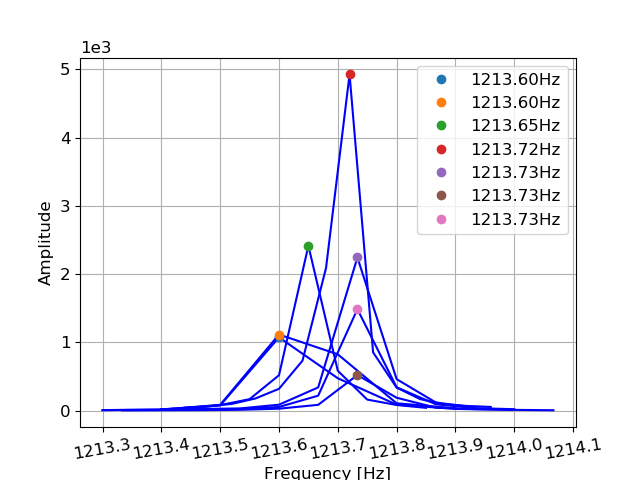
\includegraphics[width=8cm]{scripts/freq_exp2_all.png}
      \caption{Zoomed frequency plot for all 7 attempts.}
      \label{fig:sound_all}
    \end{figure}
    
    Fig. \ref{fig:sound_exp1} contains the data and derived results from our fourth attempt of the experiment. We performed a total of 7 attempts, which all yielded in similar results to attempt no. 4. The data yielded from all of the attempts is summarized in Fig. \ref{fig:sound_all} which shows the peaks in the frequency domain in one plot.
    Table \ref{tab:fftdat} contains all of the relevant numbers related to each attempt. 


    \begin{table}[H]
      % FFT DATA
      \center
      \caption{FFT data}
      \begin{tabular}{ | l | p{1.4cm} | l | l | l |}
          \hline
          Attempt no. & $f$ [Hz] & $\Delta f$ [Hz] & $t$ [s] & $f_s$ [Hz]\\ \hline
          1 & 1213.60 & 0.10 & 10 & 8192\\ \hline
          2 & 1213.60 & 0.10 & 10 & 8192\\ \hline
          3 & 1213.65 & 0.05 & 20 & 8192\\ \hline
          4 & 1213.72 & 0.04 & 25 & 8192\\ \hline
          5 & 1213.72 & 0.04 & 25 & 8192\\ \hline
          6 & 1213.72 & 0.07 & 15 & 8192\\ \hline
          7 & 1213.73 & 0.07 & 15 & 8192\\ \hline
      \end{tabular}
      \label{tab:fftdat}
    \end{table}


\newpage
\section{\label{sect:discussion}Discussion}
 
\section{\label{sect:conclusion}Conclusion}

%%%%%%%%%%%%%%%%%%%%%%%%
%%% END OF MAIN BODY %%%
%%%%%%%%%%%%%%%%%%%%%%%%

\bibliography{rapport3_ref}

\begin{thebibliography}{1}

\bibitem{squires}
G.~L. Squires.
\newblock {\em Practical Physics 4th Edition}.
\newblock Cambridge University Press, 2001.

\end{thebibliography}

\appendix*
\section{Code}
All of the code used to produce this report. Anything noteworthy should already be mentioned in the main body of the report.
\lstinputlisting[language=python]{scripts/FFTlyd.py}
\lstinputlisting[language=python]{scripts/lab_data.py}
\lstinputlisting[language=python]{scripts/FYS2150lib.py}

\end{document}